\section{Ajout d'images \addbs{tkzTabIma} et \addbs{tkzTabImaFrom}}
Ces macros permettent de placer une valeur sur une flèche de la ligne des variations. On ne peut placer une valeur que dans un intervalle où la fonction est \tkzname{monotone}, de plus l'image est celle d'un antécédent déjà défini dans la première ligne.  La première macro est \tkzcname{tkzTabIma}.

\subsection{Définition de   \addbs{tkzTabIma}}

\begin{NewMacroBox}{tkzTabIma}{\oarg{local options}\{Début\}\{Fin\}\{Position\}\{Antécédent\}\{Image\}}

\begin{tabular}{lllc}
\toprule
\texttt{arguments}   & \texttt{défaut}    & \texttt{définition}                        \\
\toprule
\IargName{tkzTabIma}{Début} & |no default|& rang de l'origine de la flèche      \\
\IargName{tkzTabIma}{Fin}  & |no default|& rang de l'extrémité de la flèche   \\
\IargName{tkzTabIma}{Position} & |no default| & rang de l'antécédent correspondant à l'image      \\
\IargName{tkzTabIma}{Image}     & |no default|  & valeur de l'image  si nécessaire     \\
\bottomrule
\end{tabular}

\medskip
\noindent\emph{Ceci mérite quelques commentaires : Il s'agit de savoir sur quelle flèche, on va positionner l'image. \tkzname{Début} et \tkzname{Fin} sont les rangs des valeurs qui déterminent les extrémités de la flèche. \tkzname{Image} est la valeur que l'on veut placer. \tkzname{Position} est un nombre entier qui est le rang de l'antécédent.}

\medskip
\begin{tabular}{lllc}
\toprule
\texttt{options}   & \texttt{défaut}    & \texttt{définition}                                      \\
\midrule
\IoptName{tkzTabIma}{draw}    & |true|   & dessin d'une flèche entre l'antécédent et son image     \\
\IoptName{tkzTabIma}{remember}& |lastval|& définit un node personnalisé                            \\
\bottomrule
\end{tabular}

\medskip
\noindent\emph{Si vous  voulez  une flèche entre l'antécédent et l'image, il vous suffit de passer en option  \tkzname{draw}. Si vous voulez référencer le point où se situe l'image alors il faut utiliser l'option \tkzname{remember}.}
\end{NewMacroBox}

\subsubsection{Ajout de valeurs intermédiaires à partir d'un antécédent donné}
Il y a plusieurs  possibilités mais la suivante est préférable. L'antécédent est de rang $2$.
 La fonction est monotone entre les valeurs de rang $1$ et $3$. Voici comment faire apparaître l'image par $f$ de $\sqrt\E$.

\begin{tkzexample}[vbox,small]
\begin{tikzpicture}
\tkzTabInit[espcl=6]%
  {$x$/1,$f'(x)$/1, $f(x)$/2}{$0$,$\sqrt\E$,$+\infty$}%
 \tkzTabLine{d,+,0,+,}%
 \tkzTabVar{D- /$-\infty$ , R /    ,+ / $0$ }%
 \tkzTabIma{1}{3}{2}{-5}
\end{tikzpicture}
\end{tkzexample}
\Iopt{tkzTabVal}{draw}

Une autre possibilité est d'utiliser la macro \tkzcname{tkzTabImaFrom} ainsi que les nodes créés pour construire le tableau ;  voir la section \og personnalisation \fg\ (\ref{pers}) et la fin de ce chapitre.

\subsubsection{Exemple avec plusieurs lignes de variations}
\begin{tkzexample}[vbox,small]
	\begin{tikzpicture}

	  \tkzTabInit[espcl=4]
	     { $x$                     /1,
	       $f''(x)$                /1,
	       $f'$                     /2,
	        Signe de\\ $f'(x)$      /2,
	       $f$                     /3}%
	     { $0$      , $1$ ,     $\alpha$,$+\infty$ }%
	  \tkzTabLine {d    , + ,   z  , -  ,      , -  }%
	  \tkzTabVar
	      {- / $1$       ,
	       + /           ,
	       R /           ,
	       - / $-\infty$ }
	  \tkzTabIma[draw]{2}{4}{3}{$0$}
    % ou bien  \tkzTabVal[draw]{2}{4}{0.5}{}{0} obsolète
    	  \tkzTabLine {     , + ,      , +  ,  z   , -  }%
	  \tkzTabVar
	     {- / $-\infty$ ,
	      R /     ,
	      + / $1$ ,
	      - / $0$       }
	  \tkzTabIma[draw]{1}{3}{2}{$0$}
	\end{tikzpicture}
\end{tkzexample}


\subsubsection{Fonctions paramétrées}
\NameFonct{Fonctions paramétrées}

\begin{tkzexample}[vbox,small]
  \begin{tikzpicture}
  \tkzTabInit[ lgt=4,  deltacl=1, espcl=2]%
    {$t$                             /1,
    Signe de\\      $x'(t)$          /1.5,
    Variations de\\ $x$              /3,
     Variations de\\  $y$            /3,
    Signe de\\ $y'(t)$              /1.5}
    { $-\infty$ , $-4$ , $-1$ , $0$, $2$ , $+\infty$}%

  \tkzTabLine { , - , z , + , d , + , z , - , d , - , }

  \tkzTabVar  {+/$1$ , -/$ \frac{8}{9}$ ,+D-/$+\infty$/$-\infty$ ,
               +/$0$/ ,-D+ /$-\infty$/ $+\infty$ , -/$1$ /   }

  \tkzTabVar  {+/$+\infty$ , R/ ,-D+/$-\infty$/$+\infty$ ,
               -/$0$ ,R / , +/$+\infty$ }

  \tkzTabIma{1}{3}{2}{$\frac{32}{3}$}
  \tkzTabIma{4}{6}{5}{$\frac{16}{3}$}

  \tkzTabLine{ , - , \frac{-64}{9} , - , d , - , z , + , \frac{44}{9} , + , }
 \end{tikzpicture}
\end{tkzexample}

\subsection{Définition de \addbs{tkzTabImaFrom}}
Cette macro ressemble à la précédente mais elle permet de placer une image relativement à une autre image ou relativement à un point quelconque du tableau auquel on a attribué un nom.

\begin{NewMacroBox}{tkzTabImaFrom}{\oarg{local options}\{Début\}\{Fin\}\{From\}\{Image\}}

\begin{tabular}{lllc}
\toprule
\texttt{arguments}   & \texttt{défaut}    & \texttt{définition}                 \\
\midrule
\IargName{tkzTabImaFrom}{Début}  & |no default|  & rang de l'origine de la flèche       \\
\IargName{tkzTabImaFrom}{Fin}  & |no default|  & rang de l'extrémité de la flèche     \\
\IargName{tkzTabImaFrom}{From}  & |no default|  & nom d'un point      \\
\IargName{tkzTabImaFrom}{Image}  & |no default|  & valeur de l'image     \\
\bottomrule
\end{tabular}

\medskip
\noindent\emph{Comme pour \tkzcname{tkzTabVal}, \tkzname{Début} et \tkzname{Fin} sont les rangs des valeurs qui déterminent les extrémités de la flèche.  \tkzname{Image} est la valeur que l'on veut placer. \tkzname{From} est  le nom du node qui correspond à l'antécédent.}

\medskip
\begin{tabular}{lllc}
\toprule
\texttt{options}   & \texttt{défaut}    & \texttt{définition}                                     \\
\midrule
\IoptName{tkzTabImaFrom}{draw}    & |true|   & dessin d'une flèche entre l'antécédent et son image     \\
\IoptName{tkzTabImaFrom}{remember}& |lastval|& définit un node personnalisé     \\
\bottomrule
\end{tabular}

\medskip
\noindent\emph{Si vous  voulez  une flèche entre l'antécédent et l'image, il vous suffit de passer en option  \tkzname{draw}. Si vous voulez référencer le point où se situe l'image alors il faut utiliser l'option \tkzname{remember}.}

\end{NewMacroBox}

\subsubsection{Utilisation d'un node défini par la macro \addbs{tkzTabInit}}
Il s'agit ici de \tkzname{N21}. C'est un node, plus exactement un point situé sous la seconde valeur $\sqrt\E$  et sur le premier filet horizontal   sous cette valeur. Voir le chapitre \tkzname{personnalisation} et en particulier l'option \tkzname{help} qui permet d'afficher différents points de construction.

\begin{tkzexample}[vbox,small]
\begin{tikzpicture}
\tkzTabInit[espcl=6]%
  {$x$/1,$f'(x)$/1, $f(x)$/3}{$0$,$\sqrt\E$,$+\infty$}%
 \tkzTabLine{d,+,0,+,}%
 \tkzTabVar{D-/      $-\infty$, R/      , +/$0$   }
 \tkzTabImaFrom[draw]{1}{3}{N21}{-5}
 \draw[opacity=0.4,fill=red!30]  (N21) circle(3ex);
 \draw[fill=red]  (N21) circle(2pt);
 \node[above right= 12pt,red](txt) at (N21) {$N21$};
\end{tikzpicture}
\end{tkzexample}
\Iopt{tkzTabImaFrom}{draw}

\subsubsection{Utilisation d'un point défini  par l'utilisateur avec \texttt{\textcolor{red}{remember}}}

\begin{tkzexample}[vbox, num,small]
	\begin{tikzpicture}
	\tkzTabInit[lgt=3,espcl=6]{ $x$/1, $f'(x)$/1, $f(x)$/3,/3 }%
	           {  $a$    , $d$    ,$e$}
	\tkzTabLine{  z,+    ,z,-     ,z  }
	\tkzTabVar  {-/\va  ,+/\vd   , -/  \ve}
	\tkzTabVal[draw,remember=vb]{1}{2}{0.333}{b}{$0$}
	\tkzTabVal[draw,remember=vc]{1}{2}{0.666}{c}{$1$}
	\tkzTabVar{-/\va  ,R/   , +/  \ve}
	\tkzTabVal[draw]{1}{3}{0.5}{}{$0$}
	\tkzTabImaFrom[draw]{1}{3}{vc}{$-1$}
	\tkzTabImaFrom[draw]{1}{3}{vb}{$-2$}
	\end{tikzpicture}
\end{tkzexample}
\Iopt{tkzTabImaFrom}{remember}

\endinput